\chapter{Tighter GSD security} \label{sec:tighter-gsd-security}

\todo{Replace \textrm{mathrm} with \textrm{operatorname} where necessary.}

\todo{Motivate GSD}

\section{Seeded GSD with Dependencies}

We call our adaptation of GSD security \emph{Seeded GSD with Dependencies} (SD-GSD). We motivate the modifications made later in Section~\vref{sec:application-to-treekem}.

\todo{Explain definition by highlighting difference to public-key GSD game.}

\todo{Motivate restrictions to the adversary.}

\todo{Do not allow cycles in $(V, E \cup D)$ either.}

\todo{Add remark that cycles are (maybe) ok in the ROM.}

\todo{Allow adversary to adaptively create nodes and seed dependencies. Also adapt proofs to guess from $[N]$ as opposed to $[n]$.}

\todo{Change proofs such that reductions simulate all ROs. Also replace $t_{H} \rightarrow x \cdot t_{\mathrm{sample}}$}

\begin{definition}[The SD-GSD game]
	Let $\lambda \in \N$ a security parameter. \question{Where to define $\lambda$?} Let $\Pi = (\gen, \enc, \dec)$ a public-key encryption scheme. Let $\hgen, \hdep \colon \{0, 1\}^\lambda \to \{0, 1\}^\lambda$ two functions. Define the game $\sdgsdgame{\Pi}$ for an adversary $\adv$:
	\begin{enumerate}[1.]
		\item \label{def:sd-gsd-game-step-1} The adversary $\adv$ outputs $n \in \N$ and a list of dependencies $D = \{(a_{i}, b_{i})\}_{i=1}^m \in [n]^2$. For each $v \in [n]$:
		      \begin{enumerate}[(i)]
			      \item \begin{itemize}
				            \item \textbf{Case $v = b_i$ for some $i$ ($v$ is the target of some dependency):} set $s_v = \hdep(s_{a_i})$.
				            \item \textbf{Otherwise:} sample $s_v \from \{0, 1\}^\lambda$.
			            \end{itemize}
			            We call $s_v$ the \emph{seed} of the node $v$ and a tuple $(a, b) \in D$ a \emph{seed dependency}.
			      \item Compute $(sk_v, pk_v) = \gen(\hgen(s_v))$. \todo{Define what RHS means.}
		      \end{enumerate}
		      Set $\mathcal{C} = E = \varnothing$. We call the directed graph $([n], E)$ a \emph{GSD graph} of \emph{size} $n$.
		\item $\adv$ may adaptively do the following queries:
		      \begin{itemize}
			      \item $\mathrm{reveal}(v)$ for $v \in [n]$: $\adv$ is given $pk_v$.
			      \item $\mathrm{encrypt}(u, v)$ for $u, v \in [n], u \neq v, (u, v) \notin E$: $(u, v)$ is added to $E$ and $\adv$ is given $c \from \enc_{pk_u}(s_v)$.
			      \item $\mathrm{corrupt}(v)$ for $v \in [n], v \notin \mathcal{C}$: $\adv$ is given $s_v$ and $v$ is added to $\mathcal{C}$. We call such a node $v \in \mathcal{C}$ \emph{corrupted}. All nodes not reachable from any corrupted node in the graph $([n], E \cup D)$ are \emph{safe} (while all other nodes are \emph{unsafe}) and we call their seeds \emph{hidden} (even if an unsafe node happens to have the same seed).
		      \end{itemize}
		\item $\adv$ outputs a node $v \in [n]$. We call $v$ the \emph{challenge node}. A bit $b \from \{0, 1\}$ is sampled and $\adv$ is given
		      \[
			      r = \begin{cases}
				      \hdep(s_v) & b = 0 \\
				      s          & b = 1
			      \end{cases},
		      \]
		      where $s \from \{0, 1\}^\lambda$. $\adv$ may continue to do queries as before.
		\item \label{def:sd-gsd-game-step-4} $\adv$ outputs a bit $b'$. The output of the game is defined to be $1$ if $b' = b$, and $0$ otherwise.
	\end{enumerate}

	We require an adversary playing the above game to adhere to the following:
	\begin{itemize}
		\item The challenge node always remains a sink \todo{Not necessary?}
		\item The challenge node is safe
		\item $\mathrm{reveal}$ is never queried on the challenge node \todo{Not necessary?}
		\item The graphs $(V, E)$ and $(V, D)$ always remain acyclic and without self-loops
		\item All paths in the graph $(V, D)$ are vertex disjoint \todo{This avoids multiple sources for single target.}
	\end{itemize}
\end{definition}


\begin{definition}[SD-GSD security]
	The triple $(\Pi, \hgen, \hdep)$, where $\Pi$ is a public-key encryption scheme and $\hgen, \hdep$ are functions $\{0, 1\}^\lambda \to \{0, 1\}^\lambda$, is \emph{$(t, \epsilon, N, \delta)$-SD-GSD secure} if for any adversary $\adv$ constructing a GSD graph of size at most $N$ and indegree at most $\delta$ and running in $t$ time we have
	\begin{align*}
		\mathrm{Adv}_{\Pi}^{\mathrm{SD-GSD}}(\adv) \coloneqq 2 \cdot \left(\pr{\mathrm{Game}_{\adv, \Pi}^{\mathrm{SD-GSD}} = 1} - \frac{1}{2}\right) \le \epsilon.
	\end{align*}
\end{definition}

Since in this work we are interested in SD-GSD security for the case where $\hgen$ and $\hdep$ are modelled as random oracles and our focus is on the encryption scheme being used, we introduce the following definition for convenience.

\begin{definition}[SD-GSD security in the ROM]
	A public-key encryption scheme $\Pi$ is \emph{$(t, \epsilon, N, \delta)$-SD-GSD secure in the ROM} if the triple $(\Pi, \hgen, \hdep)$ is $(t, \epsilon, N, \delta)$-SD-GSD secure when $\hgen$ and $\hdep$ are modelled as random oracles.
\end{definition}

\section{Proving SD-GSD security for DHIES in the ROM}

\todo{Comment on switch from IND-CPA security to EAV security.}

\begin{theorem} \label{theorem:sdgsd-security}
	Let $N, \delta \in \N$ arbitrary with $\delta \le N$. Let $\dhies$ the DHIES scheme instantiated with a private-key encryption scheme $\Pi_s$ where $\Pi_s.\gen$ samples a key uniformly at random from $\{0, 1\}^\kappa$. Let $\hdh$ the KDF and $\mathbb{G}$ the group used in $\dhies$. If $\Pi_s$ is $(t, \epsilon)$-EAV secure, the DDH problem is $(t, \epsilon)$-hard in $\mathbb{G}$ and $\hdh$ is modelled as a random oracle, then $\Pi_{\mathrm{DH}}$ is $(\tilde{t}, \tilde{\epsilon}, N, \delta)$-SD-GSD secure in the ROM with
	\[
		\tilde{\epsilon} = 2 \cdot (\delta + 1) \cdot N \cdot \epsilon + \frac{2 \cdot \mdh \cdot N^2}{\abs{\mathbb{G}}} + \frac{\ms \cdot N}{2^{\lambda - 1}},
	\]
	where $\ms$ is an upper bound on the number of queries made to either $\hgen$ or $\hdep$ and $\mdh$ is an upper bound on the number of queries made to $\hdh$, and with
	\[
		\tilde{t} = t \begin{aligned}[t]
			- & \mathcal{O}
			\begin{aligned}[t]
				\big(  \lambda & \cdot \ms \\ + & N \cdot (t_{\hgen} + t_{\hdep} + (\lambda + \kappa) \cdot t_{\mathrm{sample}} + \mdh \cdot t_{\mathrm{op}} + t_{\dhies.\gen})  \\ + & N^2 \cdot t_{\dhies.\enc}\big), \\
			\end{aligned}
		\end{aligned}
	\]
	where the various variables denote the following
	\begin{itemize}
		\item $t_{\hgen}$: time to evaluate $\hgen$ on $s \in \{0, 1\}^\lambda$
		\item $t_{\hdep}$: time to evaluate $\hdep$ on $s \in \{0, 1\}^\lambda$
		\item $t_{\mathrm{sample}}$: time to sample a bit
		\item $t_{\dhies.\enc}$: time to encrypt $s \in \{0, 1\}^\lambda$ with $\dhies$
		\item $t_{\dhies.\gen}$: runtime of $\dhies.\gen$
		\item $t_{\mathrm{op}}$: time to perform the group operation in $\mathbb{G}$
		\item $\gamma$: length of encoding of a group element $\mathbb{G}$ (used in Lemma~\ref{lemma:eav-reduction})
	\end{itemize}
\end{theorem}

\paragraph{Intuition}
Consider an arbitrary SD-GSD adversary $\adv$. For an execution of $\sdgsdgame{\dhies}$ we say ``\emph{$\adv$ wins}" to denote the event $\sdgsdgame{\dhies} = 1$.
As usual with random oracles we proceed by a case distinction on whether they were queried on some interesting value. Accordingly, let $Q_{\mathrm{x}}$ denote the event that $\adv$ queries $H_{\mathrm{x}}$ on a hidden seed for $x \in \{\mathrm{gen}, \mathrm{dep}\}$. Then we can write
\begin{align} \label{eq:theorem-sd-gsd-security-win-cases}
	\begin{split}
		\pr{\wins} & = \pr{\wins \land \qdep} + \pr{\wins \land \overline{\qdep} \,} \\
		& \le \pr{\wins \land \qdep} + \pr{\wins \mid \overline{\qdep} \,} \\
		& \stackrel{\mathclap{(\dagger)}}{=}  \pr{\wins \land \qdep} + \frac{1}{2}         \\
		& \le \pr{\qdep} + \frac{1}{2} \\
		& \le \pr{\qs} + \frac{1}{2},
	\end{split}
\end{align}
where $\qs \coloneqq \qgen \cup \qdep$ ($\mathrm{s}$ for \emph{seed}). Step $(\dagger)$ intuitively holds because without having queried $\hdep$ for any hidden seed, in particular the seed $s_v$ of the challenge node $v$, $\hdep(s_v)$ is a uniformly random value from $\adv$'s perspective. Therefore, it can do no better than guessing to distinguish $\hdep(s_v)$ from $s \from \{0, 1\}^\lambda$.

\todo{Motivate why we introduce $\qs$. (Reason: If we try to bound $\qdep$ by itself, we must separately deal with the case where the adversary was able to trigger it at a node $v$ by triggering $\qgen$ at a parent node $p$ and subsequently decrypting a ciphertext. But our argument  To eliminate this, we want to look at the point in time where either of the two events was first triggered.)}

The heart of the proof is to bound $\pr{\qs}$. When the adversary first triggers $\qs$ by querying the seed of some safe node $w$, (with overwhelming probability $w$ will be the only node with this seed and) it can only have learned the seed through encryptions
$c_1 \from \dhies.\enc_{pk_{u_1}}(s_w), \ldots, c_d \from \dhies.\enc_{pk_{u_d}}(s_w)$
where $(u_1, w), \ldots, (u_d, w)$ are edges in the GSD graph (obtained through corresponding queries $\mathrm{encrypt}(u_1, w), \ldots, \mathrm{encrypt}(u_d, w)$). The only other potential source of information about $s_w$ would be a seed dependency $(p, w)$, but this tells $\adv$ nothing: Since $w$ is safe, $p$ would also be safe and $\hdep(s_p)$ cannot have been queried due to the assumption that $w$ was the first node to trigger $\qs$.
Without having queried $\hdep(s_p)$, by virtue of $\hdep$ being a random oracle $s_w$ has the same distribution as a seed without a dependency from $\adv$'s perspective (uniformly random). See Figure~\ref{fig:gsd-qs-triggered} for an illustration of node $w$ in the GSD graph.

\begin{figure}
	\begin{center}
		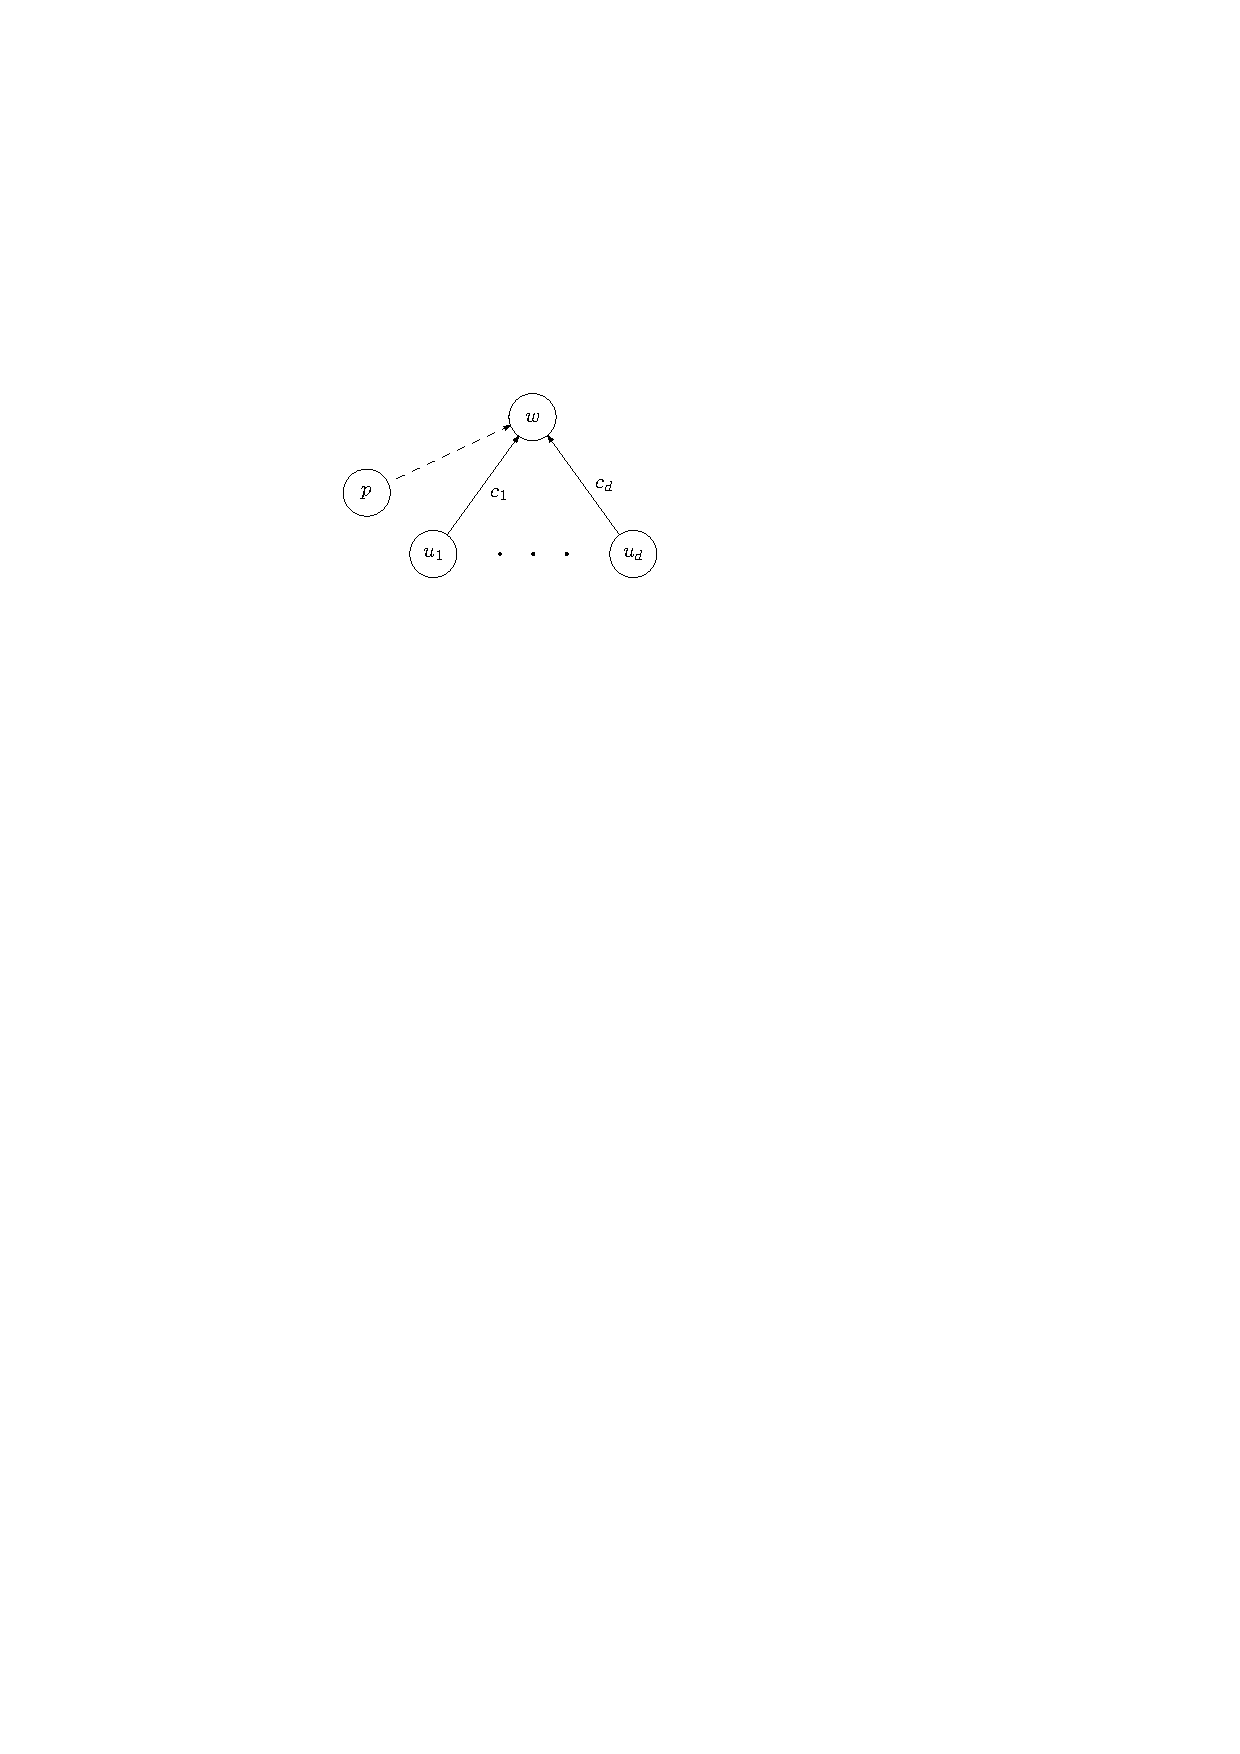
\includegraphics{figures/gsd-qs-triggered}
	\end{center}
	\caption{Illustration of the GSD graph when $\qs$ is triggered at a node $w$. The dashed edge represents a seed dependencey $(p, w)$ and the remaining edges represent encryption queries $c_i \from \mathrm{encrypt}(u_i, w)$.}
	\label{fig:gsd-qs-triggered}
\end{figure}

The proof in \cite{ttkem} simply argued that this is not too likely if these encryptions were made with an IND-CPA secure scheme. In the context of the DHIES scheme we can say more about these encryptions and achieve a better reduction loss.
Let $x_i = \log_g(pk_{u_i})$ (where $g$ is the generator of $\mathbb{G}$ being used in $\dhies$). Each encryption $c_i$ is a tuple of the form $\langle g^{y_i}, \Pi_s.\enc_{k_i}(s_w) \rangle$ where $y_i \from [\abs{\mathbb{G}}], k_i = \hdh\left(g^{x_i \cdot y_i}\right)$. Now we can again do a case distinction on whether $\hdh$ was queried for some group element $g^{x_j \cdot y_j}$ or not:
\begin{enumerate}[(i)]
	\item \label{qs-triggered-case-1} If such a query was made, then $\adv$ solved the Diffie-Hellman challenge $(g^{x_j}, g^{y_j})$. (Remember that we assumed that $w$ is the first node for which $\qs$ is triggered and as before if $w$ is safe, then so are the nodes $u_i$. Thus the adversary has not learned the exponent $x_i$ through querying $\hgen(s_{u_i})$ for any $i$.)
	\item \label{qs-triggered-case-2} If no such query was made, then from $\adv$'s perspective all the $k_i$ are independent, uniformly random keys and it still was able to learn $s_w$ from the EAV secure encryptions $\Pi_s.\enc_{k_1}(s_w), \ldots, \Pi_s.\enc_{k_d}(s_w)$.
\end{enumerate}
We can bound the probability of either of these events occurring using hardness of the DDH problem in $\mathbb{G}$ and EAV security of $\Pi_s$, respectively.

To this end, we call a group element $h \in \mathbb{G}$ a \emph{hidden Diffie-Hellman key} if $h = pk_u^{y_{u, v}}$, where $(u, v)$ is an edge in the GSD graph, $u$ is safe and $y_{u, v}$ is the exponent chosen in the DHIES encryption of $s_v$ (i.e. $\adv$ was given a ciphertext of the form $\langle g^{y_{u, v}}, \ldots\rangle$ when it queried $\mathrm{encrypt}(u, v)$). Now analogously to above let $\qdh$ the event that $\adv$ queries $\hdh$ on a hidden Diffie-Hellman key and let $\fdh$ the event that $\adv$ triggers $\qdh$ \emph{before} having triggered $\qs$. Then we can split the event $\qs$ into two cases as motivated above:
\begin{align*}
	\pr{\qs} & = \pr{\qs \land \fdh} + \pr{\qs \land \overline{\fdh}\,}.
\end{align*}
We bound $\pr{\qs \land \fdh}$ and $\pr{\qs \land \overline{\fdh} \,}$ in Lemma~\ref{lemma:dh-reduction} and Lemma~\ref{lemma:eav-reduction}, respectively. Overall this gives us a bound on the advantage of $\adv$ using \eqref{eq:theorem-sd-gsd-security-win-cases}. (To be precise, the event $\qs \land \fdh$ is a superset of case (\ref{qs-triggered-case-1}) above. However, the argument applied in Lemma~\ref{lemma:dh-reduction} gives the same bound for either event and this more general event has the advantage of being simpler.)

\begin{proof}[of Theorem~\ref{theorem:sdgsd-security}]
	Let $\adv$ an arbitrary SD-GSD adversary running in time $\tilde{t}$. We will use the events defined above. We first justify step $(\dagger)$ in \eqref{eq:theorem-sd-gsd-security-win-cases}. Note that by the rules imposed on the adversary in the SD-GSD game, the challenge node $v$ is safe and its seed $s_v$ thus indeed hidden. If $\qdep$ does not hold, then $\adv$ has not queried $\hdep$ for $s_v$ and, by virtue of $\hdep$ being a random oracle, $\hdep(s_v)$ is a uniformly distributed value in $\{0, 1\}^\lambda$ from $\adv$'s perspective. The value $s$ follows the same distribution. Thus, $\adv$ behaves the same when given either $r = s$ or $r = \hdep(s_v)$ and
	\begin{align} \label{eq:theorem-sd-gsd-security-not-qdep-behavior}
		\begin{split}
			\pr{1 \from \adv \mid \overline{\qdep}, b = 1} & = \pr{1 \from \adv \mid \overline{\qdep}, r = s}          \\
			& = \pr{1 \from \adv \mid \overline{\qdep}, r = \hdep(s_v)} \\
			& = \pr{1 \from \adv \mid \overline{\qdep}, b = 0}.
		\end{split}
	\end{align}
	Therefore
	\begin{align*}
		\pr{\wins \mid \overline{\qdep} \,} & = \begin{aligned}[t]
			                                         & \pr{1 \from \adv \mid \overline{\qdep}, b = 1} \cdot \frac{1}{2}   \\
			                                         & + \pr{0 \from \adv \mid \overline{\qdep}, b = 0} \cdot \frac{1}{2}
		                                        \end{aligned}                                                                             \\
		                                    & \stackrel{\mathclap{\eqref{eq:theorem-sd-gsd-security-not-qdep-behavior}}}{=} \begin{aligned}[t]
			                                                                                                                     & \pr{1 \from \adv \mid \overline{\qdep}, b = 0} \cdot \frac{1}{2}   \\
			                                                                                                                     & + \pr{0 \from \adv \mid \overline{\qdep}, b = 0} \cdot \frac{1}{2}
		                                                                                                                    \end{aligned} \\
		                                    & = \frac{1}{2}.
	\end{align*}

	By Lemma~\vref{lemma:dh-reduction} we have
	\[
		\pr{\qs \land \fdh} \le N \cdot \epsilon + \frac{\mdh \cdot N^2}{\abs{\mathbb{G}}}.
	\]
	and by Lemma~\vref{lemma:eav-reduction} we have
	\[
		\pr{\qs \land \overline{\fdh}\,} \le \delta \cdot N \cdot \epsilon + \frac{\ms \cdot N}{2^\lambda},
	\]
	so we know that
	\[
		\pr{\qs} \le (\delta + 1) \cdot N \cdot \epsilon + \frac{\mdh \cdot N^2}{\abs{\mathbb{G}}} + \frac{\ms \cdot N}{2^\lambda}.
	\]
	Then by \eqref{eq:theorem-sd-gsd-security-win-cases}
	\[
		\pr{\wins} \le (\delta + 1) \cdot N \cdot \epsilon + \frac{\mdh \cdot N^2}{\abs{\mathbb{G}}} + \frac{\ms \cdot N}{2^\lambda} + \frac{1}{2},
	\] so
	\[
		\mathrm{Adv}_{\Pi}^{\mathrm{SD-GSD}}(\adv) \le 2 \cdot \left((\delta + 1) \cdot N \cdot \epsilon + \frac{\mdh \cdot N^2}{\abs{\mathbb{G}}} + \frac{\ms \cdot N}{2^\lambda}\right) = \tilde{\epsilon}.
	\]
\end{proof}

\todo{Compare with result from \cite{ttkem}}.

\subsection{Reducing to EAV security}

Recall case (\ref{qs-triggered-case-2}) in the high-level discussion of Theorem~\ref{theorem:sdgsd-security}: the adversary $\adv$ was able to learn the seed $s_w$ given the EAV secure encryptions $\Pi_s.\enc_{k_1}(s_w), \ldots, \Pi_s.\enc_{k_d}(s_w)$. We can see $\adv$ as an adversary against a security game where $\adv$ is given $d$ EAV secure encryptions $c_1 \from \Pi_s.\enc_{k_1}(m), \ldots, c_d \from \Pi_s.\enc_{k_d}(m)$ of a message $m$ with $k_i \from \Pi_s.\gen()$ and must compute $m$. If we can prove that beating such a game is hard, then we can bound the probability of $\adv$ actually learning $s_w$ in this way.

This is exactly how we proceed in this section. Instead of asking the adversary to compute an encrypted message $m$, we turn to a more familiar decisional formulation as in the IND-CPA game (where the adversary may choose a pair $m_0, m_1$ and must distinguish whether the $d$ ciphertexts encrypt $m_0$ or $m_1$). We call this security notion \emph{EAV security under multiple (M) independent (I) encryptions of a single (S) pair of messages} (MIS-EAV).

\begin{definition}[The MIS-EAV game]
	Let $\Pi$ a private-key encryption scheme. Define the game $\mathrm{Game}_{\adv, \Pi}^{\mathrm{MIS-EAV}}$ for an adversary $\adv$:
	\begin{enumerate}[1.]
		\item The adversary $\adv$ outputs $q \in \N$ and a pair of messages $m_0, m_1$ of the same length. We refer to $q$ as the number of \emph{queries} made by $\adv$.
		\item A bit $b \from \{0, 1\}$ is sampled. For each $i \in [q]$, $\adv$ is given an encryption $c_i \from \Pi.\enc_{k_i}(m_b)$ where $k_i \from \Pi.\gen()$ is generated independently of the other keys.
		\item $\adv$ outputs a bit $b'$. The output of the game is defined to be $1$ if $b' = b$, and $0$ otherwise.
	\end{enumerate}
\end{definition}

\begin{definition}[MIS-EAV security]
	A private-key encryption scheme $\Pi$ is \emph{$(t, \epsilon, q)$-MIS-EAV secure} if for any adversary $\adv$ making at most $q$ queries and running in time $t$ we have
	\begin{align*}
		\mathrm{Adv}_{\Pi}^{\mathrm{MIS-EAV}}(\adv) \coloneqq 2 \cdot \left(\pr{\mathrm{Game}_{\adv, \Pi}^{\mathrm{MIS-EAV}} = 1} - \frac{1}{2}\right) \le \epsilon.
	\end{align*}
\end{definition}

Similar to how IND-CPA security for a single encryption query implies IND-CPA security for $q$ queries with a security loss of $q$ by a standard hybrid argument, one can show that EAV security implies MIS-EAV security with the same loss. To see why, recall the hybrid argument for IND-CPA security (as discussed in e.g. \cite[Theorem 12.6]{introduction-to-modern-cryptography}): We define the sequence of hybrid games $H_0, \ldots, H_q$ where in the game $H_i$ the first $i$ encryption queries encrypt the second message and the remaining $q - i$ queries encrypt the first message. Then given an IND-CPA adversary $\adv$ for multiple encryptions, an IND-CPA adversary $\adv'$ is constructed to bound
\[
	\abs*{\pr{\adv \text{ outputs } 0 \text{ in game } H_{i - 1}} - \pr{\adv \text{ outputs } 0 \text{ in game } H_{i}}}
\]
for arbitrary $i$.
The adversary $\adv'$ simulates $H_{i - 1}$ or $H_{i}$ to $\adv$ depending on whether the ciphertext received from the (single-query) IND-CPA challenger, which gets passed on as the response to the $i$-th query, encrypts the first or the second message from the $i$-th pair of messages. $\adv'$ then uses the encryption oracle to pass on the right encryptions to $\adv$ for all other queries. Now notice that if we wanted to simulate to an MIS-EAV adversary we wouldn't need access to an encryption oracle since for the MIS-EAV security game all the other encryptions can easily be generated by $\adv'$ sampling the new keys itself.

The argument would of course also work without restricting the adversary to a single pair of messages (which we could call MI-EAV security). However, we will make use of this restriction to provide a tighter reduction for a certain class of schemes at the end of this section.

\begin{lemma} \label{lemma:mis-eav-from-eav}
	Let $\Pi$ a private-key encryption scheme with finite message space. Let $t_{\gen}, t_{\enc}$ upper bounds for the runtime of $\Pi.\gen$ and $\Pi.\enc$, respectively. If $\Pi$ is $(t, \epsilon)$-EAV secure, then for all $q \in \N$, $\Pi$ is $(\tilde{t}, q \cdot \epsilon, q)$-MIS-EAV secure with $\tilde{t} = t - \mathcal{O}(q \cdot (t_\gen + t_\enc))$.
\end{lemma}

The details of the proof can be found in Section~\ref{sec:mis-eav-from-eav-proof} of the appendix.

\begin{lemma} \label{lemma:eav-reduction}
	Recall the assumptions, variables and events from the statement and proof of Theorem~\ref{theorem:sdgsd-security}. In particular, assume that $\Pi_s$ is $(t, \epsilon)$-EAV secure. Let $\adv$ an SD-GSD adversary running in time $\tilde{t}$, making at most $\ms$ queries to $\hgen$ or $\hdep$ and at most $\mdh$ queries to $\hdh$. Then
	\[
		\pr{\qs \land \overline{\fdh}\,} \le \delta \cdot N \cdot \epsilon + \frac{\ms \cdot N}{2^\lambda}.
	\]
\end{lemma}

\paragraph{Intuition} By Lemma~\vref{lemma:mis-eav-from-eav} we know that $\Pi_s$ is MIS-EAV secure. Continuing the high-level argument before the proof of Theorem~\ref{theorem:sdgsd-security}, consider the first moment that $\adv$ triggers $\qs \land \overline{\fdh}$ by querying the seed of some safe node $w$.  As intended, it follows from the definition of the event $\fdh$ that from $\adv$'s perspective all DHIES ciphertexts it got from queries $\mathrm{encrypt}(u, w)$ for any $u$ contain encryptions of $s_w$ under independent, uniformly random keys using $\Pi_s$. Moreover, as already argued once, $\adv$ has learned nothing from a potential seed dependency $(p, w)$, so these encryptions are everything $\adv$ had at its proposal to learn $s_w$.

\todo{Add plot.}

We can use $\adv$'s ability to compute the seed $s_w$ of a safe node $w$ from encryptions of $s_w$ to construct an MIS-EAV adversary: We first guess a node $w$ whose seed $\adv$ may query. Next we give the MIS-EAV challenger $s_w$ and some other independent seed $s$, and embed the encryptions we get back into the SD-GSD game when answering queries of the form $\mathrm{encrypt}(u, w)$ for any $u$. Now consider the behavior of $\adv$ depending on which seed the challenger chooses to encrypt:
\begin{itemize}
	\item If the challenger chooses to encrypt $s_w$, then $\adv$ will trigger the event $\qs \land \overline{\fdh}$ with the same probability as before and if we guessed $w$ correctly we can detect whether $\qs \land \overline{\fdh}$ gets triggered (by checking if $\hgen(s_w)$ or $\hdep(s_w)$ was queried by $\adv$ during the simulation).
	\item If the challenger chooses to encrypt $s$, then $\adv$ receives no information about $s_w$ and has negligible probability of querying it.
\end{itemize}
Thus, the advantage of the adversary is about $\pr{\qs \land \overline{\fdh}\,}/N$, where the factor $1/N$ arises from guessing $w$, and using that $\Pi_s$ is MIS-EAV secure we can bound this probability. Since we are only interested in checking whether the event was triggered for $w$, the adversary can abort when this is no longer possible ($w$ is corrupted, some other hidden seed is queried, etc.).

\begin{proof}[of Lemma~\ref{lemma:eav-reduction}]
	As motivated above we construct an MIS-EAV adversary $\adv'$ to derive the bound. $\adv'$ behaves as follows:
	\begin{enumerate}[1.]
		\item $\adv'$ runs $\adv$ to get $n$ and $D$ and initializes the GSD graph, seeds and the set of edges and corrupted nodes as in step \ref{def:sd-gsd-game-step-1} of the SD-GSD game.
		\item $\adv'$ samples $w \from [n], s \from \{0, 1\}^\lambda$ and gives $\delta$ and the messages $s_w, s$ to the challenger. Let $c_1, \ldots, c_\delta$ the encryptions it gets back.
		\item $\adv'$ faithfully simulates the SD-GSD game to $\adv$ with the following exception: Whenever $\adv$ makes a query of the form $\mathrm{encrypt}(u, w)$ for any $u$, $\adv'$ replies with $\langle g^x, c_i \rangle$ where $x \from [\abs{\mathbb{G}}]$ and $i$ is the index of the next ciphertext (from step 2) not yet used.

		      During the simulation $\adv'$ also pays attention to the following:
		      \begin{itemize}
			      \item If any of the following events occur, $\adv'$ aborts the simulation and outputs 1:
			            \begin{itemize}
				            \item $\adv$ queries $\hdh$ for a hidden Diffie-Hellman key
				            \item $\adv$ queries $\hgen$ or $\hdep$ for a hidden seed that is not $s_w$
				            \item $\adv$ queries $\mathrm{corrupt}(u)$ for some node $u$ such that $w$ is no longer safe
			            \end{itemize}
			      \item If $\adv$ queries $\hgen(s_w)$ or $\hdep(s_w)$, $\adv'$ aborts the simulation and outputs 0. This is the only point at which $\adv'$ outputs 0.
		      \end{itemize}

		      If the simulation arrives to the point where $\adv$ outputs its guess (step \ref{def:sd-gsd-game-step-4} of the SD-GSD game), then $\adv'$ outputs 1.
	\end{enumerate}

	The advantage of $\adv'$ is given by
	\begin{equation} \label{eq:lemma-eav-reduction-advantage}
		\mathrm{Adv}_{\Pi}^{\mathrm{MIS-EAV}}(\adv') \stackrel{\eqref{eq:advantage-equality}}{=}  \pr{0 \from \adv' \mid b = 0} - \pr{0 \from \adv' \mid b = 1},
	\end{equation}
	where $b$ is the bit sampled by the MIS-EAV challenger.


	First, we will show that
	\begin{equation} \label{eq:lemma-eav-reduction-b=0}
		\pr{0 \from \adv' \mid b = 0} \ge \frac{\pr{\qs \land \overline{\fdh}\,}}{N}.
	\end{equation}
	Let $E = \qs \land \overline{\fdh}$ and let $E'$ the same event in the SD-GSD game simulated to $\adv$ during an execution of $\mathrm{Game}_{\adv', \Pi_s}^{\mathrm{MIS-EAV}}$ with $b = 0$. In the following while showing \eqref{eq:lemma-eav-reduction-b=0} we will implicitly assume that $b = 0$ when referring to the game simulated to $\adv$ by $\adv'$.
	On a high level \eqref{eq:lemma-eav-reduction-b=0} holds due to the fact that as long as the game has not been aborted the encryptions $\adv$ receives from $\adv'$ are indistinguishable from what it would get in the real SD-GSD game and we get a factor $\frac{1}{N}$ from guessing the node that triggered $E$. However, showing this requires a few steps.

	Consider a modification of the SD-GSD game $G_1$ where the game is aborted whenever one of the following events occurs, where for all these events $\adv'$ would also abort the simulation:
	\begin{itemize}
		\item $\adv$ queries $\hdh$ for a hidden Diffie-Hellman key
		\item $\adv$ queries $\hgen$ or $\hdep$ for a hidden seed
	\end{itemize}
	(Since we are not interested in the output of the game we can define \emph{aborting the game} as the game ending with output 0.) The game $G_1$ is something between the real SD-GSD game and what $\adv'$ simulates to $\adv$. The only difference in when $G_1$ aborts compared to the game simulated by $\adv'$ is that we aren't paying attention to some specific node $w$ remaining safe. Aborting the game in this way does not alter the probability of $\adv$ triggering the event $E$ in $G_1$, since in either case when the game is aborted either $E$ or $\overline{E}$ is already known to hold:
	\begin{itemize}
		\item If $\adv$ queries $\hdh$ for a hidden Diffie-Hellman key, then it triggers $\qdh$ and $\qs$ has not been triggered before since this would have caused the game to be aborted. Thus, $\adv$ triggered $\fdh$ and $\qs \land \overline{\fdh}$ cannot hold in this execution of the game.
		\item If $\adv$ queries $\hgen$ or $\hdep$ for a hidden seed, then this triggers $\qs$. Moreover, $\overline{\fdh}$ also holds at this moment since the game would have aborted earlier if $\qdh$ had already been triggered. Thus, $\qs \land \overline{\fdh}$ holds.
	\end{itemize}
	Let $E_1$ the same event as $E$ in the game $G_1$. As argued above we have
	\begin{equation} \label{eq:lemma-eav-reduction-E=E_1}
		\pr{E_1} = \pr{E}.
	\end{equation}


	Now consider a game $G_2$ which is a modification of the game $G_1$ where at the beginning of the game $w_2 \from [n]$ is sampled and the game also aborts if $\adv$ queries $\mathrm{corrupt}(u)$ for some node $u$ such that $w_2$ is no longer safe, just as in the game simulated by $\adv'$. The game $G_2$ is again something between the game $G_1$ and what $\adv'$ simulates to $\adv$. We also modify $G_1$ such that it also samples $w_1 \from [n]$ at the beginning of the game. This does not change the fact that \eqref{eq:lemma-eav-reduction-E=E_1} holds as the sampling of $w_1$ has no effect on the execution of the game.

	Let $E_2$ and $E'$ the events corresponding to $E$ in the game $G_2$ and the game simulated by $\adv'$, respectively. We further introduce a new random variable $W$ to analyze each game where
	\[
		W = \begin{cases}
			0 & \overline{E}                       \\
			x & E \text{ was triggered at node } x
		\end{cases}
	\]
	(if $x$ is not unique we choose the node with lowest identifier).
	Let $W_1$, $W_2$ and $W'$ be the corresponding random variables in game $G_1$, game $G_2$ and the game simulated by $\adv'$. Consider the probability $\pr{W_1 = w_1 \mid E_1}$. The node $w_1$ is sampled independently and does not affect the execution of the game. Therefore, in an execution where $E_1$ occurs and the GSD graph has size $n$ (so $W_1 \in [n]$), we correctly guess $W_1 = w_1$ with probability exactly $\frac{1}{n} \ge \frac{1}{N}$. Thus
	\[
		\pr{W_1 = w_1 \mid E_1} \ge \frac{1}{N}
	\]
	and combining this with \eqref{eq:lemma-eav-reduction-E=E_1} we get
	\begin{align} \label{eq:lemma-eav-reduction-detect-E1-G1}
		\begin{split}
			\pr{W_1 = w_1} & = \pr{W_1 = w_1 \land E_1} \\
			& = \pr{W_1 = w_1 \mid E_1} \cdot \pr{E_1} \\
			& \ge \frac{1}{N} \cdot \pr{E}.
		\end{split}
	\end{align}

	Analogously to the argument used to justify \eqref{eq:lemma-eav-reduction-E=E_1}, we can argue that
	\begin{equation} \label{eq:lemma-eav-reduction-G1-vs-G2}
		\pr{W_1 = w_1} = \pr{W_2 = w_2}.
	\end{equation}
	The only difference from $G_1$ to $G_2$ is that $G_2$ aborts when $w_2$ is no longer safe. But if $w_2$ is no longer safe then we know that $W_2 \neq w_2$ (if $W_2 = w_2$ the game would have already aborted when $w_2$'s seed was queried while it was safe). Thus, \eqref{eq:lemma-eav-reduction-E=E_1} indeed holds.

	We now show an analogous result comparing the game $G_2$ to the game simulated by $\adv'$:
	\begin{equation} \label{eq:lemma-eav-reduction-G2-vs-simulation}
		\pr{W_2 = w_2} = \pr{W' = w}.
	\end{equation}
	Consider how $G_2$ differs from the game simulated by $\adv'$. Both games abort at exactly the same events (verify this! \question{Ok to add such a note for the reader?}). They only differ in how $\adv'$ answers queries $\mathrm{encrypt}(u, w)$ for any $u$. In $G_2$ such a query is answered with a ciphertext $\langle g^x, c \rangle$ where $x \from [\abs{\mathbb{G}}], c \from \Pi_s.\enc_k(s_w)$ and $k = \hdh(pk_u^x)$. $\adv'$ answers such a query with $\langle g^{x'}, c' \rangle$ where $x' \from [\abs{\mathbb{G}}], c' \from \Pi_s.\enc_{k'}(s_w)$ and $k' \from \{0, 1\}^\kappa$. Now notice that as long as the game $G_2$ is ongoing, $pk_u^{x}$ is a hidden Diffie-Hellman key and $\adv$ has not queried $pk_u^{x}$ to $\hdh$. If it had, then the game would have already aborted. Therefore, from $\adv$'s view $k$ follows the same distribution as $k'$. Thus, overall the game $G_2$ and the game simulated by $\adv'$ are indistinguishable to $\adv$ and \eqref{eq:lemma-eav-reduction-G2-vs-simulation} holds.

	Finally, notice that if the event $W' = w$ occurred, then $\adv'$ outputs $1$. Then we have
	\begin{align*}
		\pr{1 \from \adv' \mid b = 0} & \ge \pr{W' = w}                                                              \\
		                              & \stackrel{\eqref{eq:lemma-eav-reduction-G2-vs-simulation}}{=} \pr{W_2 = w_2} \\
		                              & \stackrel{\eqref{eq:lemma-eav-reduction-G1-vs-G2}}{=}  \pr{W_1 = w_1}        \\
		                              & \stackrel{\eqref{eq:lemma-eav-reduction-detect-E1-G1}}{\ge} \frac{\pr{E}}{N} \\
		                              & = \frac{\pr{\qs \land \overline{\fdh}\,}}{N},
	\end{align*}
	as promised.

	Second, returning to \eqref{eq:lemma-eav-reduction-advantage}, we can more easily show that $\pr{0 \from \adv' \mid b = 1}$ is negligible. In the SD-GSD game simulated to $\adv$ during an execution of $\mathrm{Game}_{\adv', \Pi_s}^{\mathrm{MIS-EAV}}$ with $b = 1$, the seed $s_w$ is a random variable independent of any information given to $\adv$:
	\begin{itemize}
		\item the game aborts when $w$ becomes unsafe, so $s_w$ cannot be learned by querying $\mathrm{corrupt}(w)$ or by querying $\hdep(s_p)$ for an unsafe node $p$ where $(p, w)$ is a seed dependency
		\item querying $\hdep(s_p)$ for a safe node $p$ where $(p, w)$ is a seed dependency results in the game being aborted and by virtue of $\hdep$ being a random oracle, from $\adv$'s perspective $s_w$ follows the same distribution regardless of whether there is a seed dependency $(p, w)$ or not
		\item with $b = 1$ queries $\mathrm{encrypt}(u, w)$ yield encryptions of $s$ instead of $s_w$
	\end{itemize}
	Therefore, for any seed $s'$ that $\adv$ queries to $\hgen$ or $\hdep$ we have
	\[
		\pr{s_w = s'} = \frac{1}{2^\lambda}.
	\]
	Thus, by a union bound we have
	\begin{equation} \label{eq:lemma-eav-reduction-b=1}
		\pr{0 \from \adv' \mid b = 1} \le \frac{\ms}{2^\lambda}.
	\end{equation}

	Combining \eqref{eq:lemma-eav-reduction-advantage}, \eqref{eq:lemma-eav-reduction-b=0} and \eqref{eq:lemma-eav-reduction-b=1} we get
	\begin{align} \label{eq:lemma-eav-reduction-advantage-lower-bound}
		\begin{split}
			\mathrm{Adv}_{\Pi}^{\mathrm{MIS-EAV}}(\adv') & = \pr{0 \from \adv' \mid b = 0} - \pr{0 \from \adv' \mid b = 1}           \\
			& \ge \frac{\pr{\qs \land \overline{\fdh}\,}}{N} - \frac{\ms}{2^\lambda}.
		\end{split}
	\end{align}
	Furthermore, going through the details yields that $\adv'$ runs in time
	\begin{align*}
		\begin{split}
			t_{\adv'} \coloneqq \tilde{t} + \mathcal{O}\big(\lambda \cdot \ms & +  \gamma \cdot \mdh  \\
			& + N \cdot (t_{\hgen} + t_{\hdep} + \lambda \cdot t_{\mathrm{sample}} + t_{\dhies.\gen})  \\
			& +  N^2 \cdot t_{\dhies.\enc}\big)
		\end{split}
	\end{align*}
	(the simulation of the SD-GSD game dominating the additional runtime).
	Using that $t_{\mathrm{op}} = \Omega(\gamma), \delta \le N, t_{\Pi_s.\gen} = \mathcal{O}(\kappa \cdot t_{\mathrm{sample}})$, $t_{\Pi_s.\enc} \le t_{\dhies.\enc}$ (as encrypting with $\dhies$ involves an encryption with $\Pi_s$) and the definition of $\tilde{t}$, with appropriately chosen constants we have
	\[
		t_{\adv'} \le t - \mathcal{O}(\delta \cdot (t_{\Pi_s.\gen} + t_{\Pi_s.\enc})).
	\]

	By Lemma~\ref{lemma:mis-eav-from-eav} $\Pi_s$ is $(t - \mathcal{O}(\delta \cdot (t_{\Pi_s.\gen} + \Pi_s.\enc)), \delta \cdot \epsilon, \delta)$-MIS-EAV secure, so
	\begin{equation} \label{eq:lemma-eav-reduction-advantage-upper-bound}
		\mathrm{Adv}_{\Pi}^{\mathrm{MIS-EAV}}(\adv') \le \delta \cdot \epsilon.
	\end{equation}

	Finally, if we now combine \eqref{eq:lemma-eav-reduction-advantage-lower-bound} and \eqref{eq:lemma-eav-reduction-advantage-upper-bound} we get
	\begin{align*}
		\frac{\pr{\qs \land \overline{\fdh}\,}}{N} - \frac{\ms}{2^\lambda} & \le \delta \cdot \epsilon                                          \\
		                                                                   & \iff                                                               \\
		\pr{\qs \land \overline{\fdh}\,}                                   & \le \delta \cdot N \cdot \epsilon + \frac{\ms \cdot N}{2^\lambda},
	\end{align*}
	as was to prove.
\end{proof}

\subsubsection{Tighter MIS-EAV security for certain schemes} \label{sec:tighter-mis-eav-security}

In our reduction from MIS-EAV security to EAV security (Lemma~\ref{lemma:mis-eav-from-eav}) we applied a general hybrid argument. It is also tempting to try a more direct approach. The EAV and MIS-EAV games seem less far apart than IND-CPA for single and multiple encryptions: All additional encryptions in the MIS-EAV game encrypt the same message, with the only difference being that each encryption is performed using a fresh key. If only we could take a single encryption $c \from \enc_k(m)$ and from it produce several encryptions $c_i \from \enc_{k_i}(m)$ for $k_i \from \gen()$ (without knowing $k$ or $m$), then the additional encryptions would leak no new information to the adversary, and we would have a tight bound on MIS-EAV security from EAV security. There is a simple EAV secure scheme that achieves the above property: the one-time pad. Given an encryption $c = k \oplus m$, we can just sample $k' \from \{0, 1\}^\kappa$ and compute the ciphertext $c' = c \oplus k' = (k \oplus k') \oplus m$, an encryption of $m$ under the uniformly random key $k \oplus k'$. In the following, we formalize this property of a private-key encryption scheme and use it to prove the desired bound on MIS-EAV security.

\begin{definition}[Key-rerandomizability] \label{def:key-rerandomizability}
	Let $\Pi$ a private-key encryption scheme with security parameter $\kappa$. $\Pi$ is \emph{key-rerandomizable} if there exists a probabilistic polynomial time algorithm $\mathrm{ReRan}$ achieving the following: Given $c \from \enc_k(m)$ for any fixed message $m$ in the message space and $k \from \gen()$, the output $c' \from \mathrm{ReRan}(c)$ follows the same distribution as the process of sampling $k' \from \gen()$ and computing a ciphertext $\enc_{k'}(m)$. The runtime must be polynomial in $\kappa$ and the length of the ciphertext $c$.
\end{definition}

\paragraph{Example} As outlined above, the one-time pad is an example of a key-rerandomizable encryption scheme.

\question{Is there a key-rerandomizable IND-CPA secure scheme? If yes, this would imply a key-rerandomizable AE scheme using the encrypt-then-authenticate paradigm, since a rerandomized tag can easily produced for the ciphertext by sampling a fresh MAC key.}

The key idea underlying the proof of the following Lemma was already provided at the beginning of this section.

\begin{lemma} \label{lemma:mis-eav-from-eav-with-key-rerandomizability}
	Let $\Pi$ a key-rerandomizable private-key encryption scheme with finite message space. Let $\mathrm{ReRan}$ the corresponding algorithm to rerandomize ciphertexts and $t_{\mathrm{ReRan}}$ an upper bound for the runtime of $\mathrm{ReRan}$. If $\Pi$ is $(t, \epsilon)$-EAV secure, then for all $q \in \N$, $\Pi$ is $(\tilde{t}, \epsilon, q)$-MIS-EAV secure with $\tilde{t} = t - \mathcal{O}(q \cdot t_{\mathrm{ReRan}})$.
\end{lemma}

\begin{proof}
	Note that since the message space and thus the ciphertext space is finite, the runtime of $\mathrm{ReRan}$ is indeed bounded. Let $\adv$ an MIS-EAV adversary running in time $\tilde{t}$ and making at most $q$ queries. We construct an EAV adversary $\adv'$ that behaves as follows:
	\begin{enumerate}[1.]
		\item $\adv'$ runs $\adv$ to get the number of queries $q$ and messages $m_0, m_1$.
		\item $\adv'$ gives $m_0, m_1$ to the challenger and receives. Let $c_1$ the ciphertext it gets back.
		\item $\adv'$ computes ciphertexts $c_2 \from \mathrm{ReRan}(c_1), \ldots, c_q \from \mathrm{ReRan}(c_1)$ (with independent runs of $\mathrm{ReRan}$).
		\item $\adv'$ gives the ciphertexts $c_1, \ldots, c_q$ to $\adv$.
		\item $\adv'$ outputs whatever bit $\adv$ outputs.
	\end{enumerate}
	We apply the properties of $\mathrm{ReRan}$ given in Definition~\ref{def:key-rerandomizability} to show that the game simulated to $\adv$ is distributed identically to the MIS-EAV game. For this we need only show that the ciphertexts $c_1, \ldots, c_q$ given to $\adv$ in the simulation are distributed identically to the ciphertexts $c_1', \ldots, c_q'$ that $\adv$ would get in the real MIS-EAV game. It is immediate that $c_1$ is distributed identically to $c_1'$. Now let $i \in \{2, \ldots, q\}$. By Definition~\ref{def:key-rerandomizability} $\mathrm{ReRan}(c)$ outputs a ciphertext encrypting $m_b$ (where $b$ is the bit chosen by the EAV challenger) distributed identically to a ciphertext encrypting $m_b$ output by the MIS-EAV challenger. Thus, indeed for any $i$, $c_i$ is distributed identically to $c_i'$ and the claim holds. Therefore
	\begin{equation} \label{eq:lemma-key-rerandomizability-advantage-same}
		\mathrm{Adv}_{\Pi}^{\mathrm{MIS-EAV}}(\adv) = \mathrm{Adv}_{\Pi}^{\mathrm{EAV}}(\adv').
	\end{equation}

	Because $\adv'$ is an EAV adversary running in time $\tilde{t} + \mathcal{O}(q \cdot t_{\mathrm{ReRan}}) = t$ we know that
	\[
		\mathrm{Adv}_{\Pi}^{\mathrm{EAV}}(\adv') \le \epsilon,
	\]
	which together with \eqref{eq:lemma-key-rerandomizability-advantage-same} concludes the proof.
\end{proof}

By assuming a key-rerandomizable encryption scheme and applying Lemma~\vref{lemma:mis-eav-from-eav-with-key-rerandomizability} instead of the hybrid argument (Lemma~\ref{lemma:mis-eav-from-eav}) in the proof of Lemma~\ref{lemma:eav-reduction}, we can drop the $\delta$ factor in the bound. This also allows us to drop the $\delta$ factor in Theorem~\vref{theorem:sdgsd-security}.

\begin{corollary}
	Recall the setting of Theorem~\ref{theorem:sdgsd-security}. If the private-key encryption scheme $\Pi_s$ is additionally key-rerandomizable, then the bound in Lemma~\ref{lemma:eav-reduction} can be improved to
	\[
		\pr{\qs \land \overline{\fdh}\,} \le N \cdot \epsilon + \frac{\ms \cdot N}{2^\lambda}
	\]
	and the bound $\tilde{\epsilon}$ on the success probability of an SD-GSD adversary thus improved to
	\[
		\tilde{\epsilon} = 4 \cdot N \cdot \epsilon + \frac{2 \cdot \mdh \cdot N^2}{\abs{\mathbb{G}}} + \frac{\ms \cdot N}{2^{\lambda - 1}}
	\]
	(with appropriate changes to the runtime $\tilde{t}$).
\end{corollary}


\subsection{Reducing to the DDH problem}

\begin{lemma} \label{lemma:dh-reduction}
	Recall the assumptions, variables and events from the statement and proof of Theorem~\ref{theorem:sdgsd-security}. In particular, assume that the DDH problem is $(t, \epsilon)$-hard in $\mathbb{G}$. Let $\adv$ an SD-GSD adversary running in time $\tilde{t}$, making at most $\ms$ queries to $\hgen$ or $\hdep$ and at most $\mdh$ queries to $\hdh$. Then
	\[
		\pr{\qs \land \fdh} \le N \cdot \epsilon + \frac{\mdh \cdot N^2}{\abs{\mathbb{G}}}.
	\]
\end{lemma}

\paragraph{Intuition} We will bound the simpler event $\fdh$. This event tells us that there is some safe node $a$ in the GSD graph with encryption edges to nodes $u_1, \ldots, u_d$, where the query $\mathrm{encrypt}(a, u_i)$ returned the ciphertext $\langle g^{y_i}, \enc_{k_i}(s_{u_i}) \rangle$ with $k_i = \hdh(g^{sk_{a} \cdot y_i})$, such that $g^{sk_a \cdot y_j}$ was the first hidden Diffie-Hellman key queried by $\adv$ for some $j$.
Moreover, at the instance $g^{sk_a \cdot y_j}$ was queried, no hidden seed had yet been queried by $\adv$, implying that $\adv$ had not queried $\hgen(s_a)$ and thus had no information about $sk_a$ (recall that $(pk_a, sk_a) = \gen(\hgen(s_a))$).

\todo{Add plot.}

It is interesting to note that our approach does not require that $\adv$ has not queried $\hdep$ for a hidden seed (i.e. that $\qdep$ was not triggered) as is implied by the event $\fdh$, because knowing $\hgen(s_a)$ is the only way to learn about $sk_a$. Regardless, we still want to have our definition of $\fdh$ include this information, as the bound on $\pr{\qs \land \overline{\fdh} \,}$ in Lemma~\vref{lemma:eav-reduction} relies on the fact that in the event of $\qs \land \overline{\fdh}$ happening,  $\qdh$ was not yet triggered when the event $\qs$ was triggered, i.e. when either the event $\qgen$ \emph{or} the event $\qdep$ was triggered.

The intuition is clear that this means that $\adv$ solved the Diffie-Hellman challenge $(g^{sk_a}, g^{y_j})$. What is not immediately clear is how to embed a \emph{given} Diffie-Hellman challenge $(g^x, g^y)$  from an instance of the DDH game and use $\adv$ to tell whether the key $k$ chosen by the challenger is the real key $g^{x \cdot y}$ or a uniformly random group element.
An intuitive strategy would be to embed the challenge by setting $pk_a = g^x$ and $g^{y_j} = g^y$, which involves guessing $u_j$, and simply checking whether for any of the queries $q_i$ to $\hdh$ by $\adv$ it holds that $q_i = k$. Now:
\begin{itemize}
	\item If $k = g^{x \cdot y}$, $\adv$ triggers $\fdh$ and we guessed $a$ and $u_j$ correctly, then indeed as described above $q_i = g^{sk_a \cdot y_j} = k$ will hold for some $i$.
	\item If $k$ is a random group element, then $\adv$ has negligible probability of querying $k$, as no information about $k$ is ever leaked to $\adv$.
\end{itemize}
If we make sure not to change $\adv$'s view of the game in the case $k = g^{x \cdot y}$ in this process, we can achieve an advantage of about $\pr{\fdh} / N^2$, where one factor $1/N$ arises from guessing $a$ and another from guessing $u_j$. Unfortunately, this would yield no improvement over the result from \cite{ttkem}.

\question{How to clarify that this was not my idea?} We can avoid guessing $u_j$ by being more clever about how we embed $g^y$. Instead of embedding $g^y$ into a single encryption edge, we embed it into all encryption edges. To get a uniformly random exponent from $y$ we set $y_j = y + r_j \mod \abs{\mathbb{G}}$ with $r_j \from [\abs{\mathbb{G}}]$. Given $g^{x \cdot y_j}$, we can easily compute $g^{x \cdot y}$:
\[
	g^{x \cdot y_j} = g^{x \cdot (y + r_j)} = g^{x \cdot y}	\cdot g^{x \cdot r_j} \iff g^{x \cdot y} = g^{x \cdot y_j} \cdot \underbrace{((g^x)^{r_j})^{-1}}_{\eqqcolon \, R_j}.
\]
Now to determine whether $k$ is the real Diffie-Hellman key, we check whether $q_i \cdot R_j = k$ for some $i, j$. This yields an advantage of about $\pr{\fdh} / N$ (and a slightly larger runtime). We can now proceed with the full proof.

\begin{proof}[of Lemma~\ref{lemma:dh-reduction}]
	As outlined above we use $\adv$ to construct a DDH adversary $\adv'$.
	\begin{enumerate}[1.]
		\item $\adv'$ gets $h_1, h_2$ and $k$ from the DDH challenger.
		\item $\adv'$ runs $\adv$ to get $n$ and $D$, samples $a \from [n]$ and initializes the GSD graph, seeds and the set of edges and corrupted nodes as in step \ref{def:sd-gsd-game-step-1} of the SD-GSD game, with the sole exception that $pk_a = h_1$ (as opposed to setting it to the public key output from $\gen(\hgen(s_a))$).
		\item $\adv'$ faithfully simulates the SD-GSD game to $\adv$ with the following exception: For the $j$-th query $\mathrm{encrypt}(a, u_j)$ made by $\adv$, $\adv'$ replies with $\langle h_2 \cdot g^{r_j}, \enc_{k_j}(s_{u_j}) \rangle$ where $r_j \from [\abs{\mathbb{G}}]$, $k_j \from \{0, 1\}^\kappa$. $\adv'$ also computes and stores $R_j = \left(pk_a^{r_j}\right)^{-1}$.

		      During the simulation $\adv'$ also pays attention to the following:
		      \begin{itemize}
			      \item If any of the following events occur, $\adv'$ aborts the simulation and outputs 1:
			            \begin{itemize}
				            \item $\adv$ queries $\hdh$ for a hidden Diffie-Hellman key on an encryption edge $(u, v) \in E$ with $u \neq a$
				            \item $\adv$ queries $\hgen$ or $\hdep$ for a hidden seed
				            \item $\adv$ queries $\mathrm{corrupt}(u)$ for some node $u$ such that $a$ is no longer safe
			            \end{itemize}
			      \item If $\adv$ queries $q_i$ to $\hdh$ such that $q_i \cdot R_j = k$ for some $j$, $\adv'$ aborts the simulation and outputs 0. This is the only point at which $\adv'$ outputs 0.
		      \end{itemize}

		      If the simulation arrives to the point where $\adv$ outputs its guess (step \ref{def:sd-gsd-game-step-4} of the SD-GSD game), then $\adv'$ outputs 1.
	\end{enumerate}

	The advantage of $\adv'$ is given by
	\begin{equation} \label{eq:lemma-dh-reduction-advantage}
		\mathrm{Adv}_{(\mathbb{G}, g)}^{\mathrm{DDH}}(\adv') \stackrel{\eqref{eq:advantage-equality}}{=} \pr{0 \from \adv' \mid b = 0} - \pr{0 \from \adv' \mid b = 1},
	\end{equation}
	where $b$ is the bit sampled by the DDH challenger.

	First, we will show that
	\begin{equation} \label{eq:lemma-dh-reduction-b=0}
		\pr{0 \from \adv' \mid b = 0} \ge \frac{\pr{\fdh}}{N}.
	\end{equation}
	This part of the proof proceeds very similarly to the proof of Lemma~\vref{lemma:eav-reduction} and we will be a bit more concise. We focus on executions of $\mathrm{Game}_{\adv, (\mathbb{G}, g)}^{\mathrm{DDH}}$ with $b = 0$. Let the games $G_1, G_2$ be defined as in Lemma~\ref{lemma:eav-reduction}, where we denote the node sampled at the beginning of each game by $a_1, a_2$, respectively (as opposed to $w_1, w_2$). Let $E = \fdh$ and let $E_1, E_2$ and $E'$ be the analogous events in $G_1, G_2$ and the game simulated by $\adv'$ (note that in this latter game, the group elements $pk_a^{\log_g(h_2) + r_j}$ are also hidden Diffie-Hellman keys). Finally, we introduce the random variable
	\[
		A = \begin{cases}
			0 & \overline{\fdh}                                                                    \\
			x & \text{$\fdh$ holds and $\qdh$ was triggered on an encryption edge with source $x$}
		\end{cases}
	\]
	(if $x$ is not unique we choose the node with smallest identifier) and let $A_1, A_2$ and $A'$ denote the corresponding random variables in game $G_1$, game $G_2$ and the game simulated by $\adv'$.

	Just as argued in Lemma~\ref{lemma:eav-reduction},
	\begin{equation} \label{eq:lemma-dh-reduction-E=E_1}
		\pr{E_1} = \pr{E}
	\end{equation}
	holds, since whenever $G_1$ aborts, it is already decided whether $\fdh$ holds:
	\begin{itemize}
		\item If the game was aborted when $\adv$ queried a hidden Diffie-Hellman key, then $\fdh$ holds.
		\item If the game was aborted when $\adv$ queried $\hgen$ or $\hdep$ for a hidden seed, $\fdh$ does not hold.
	\end{itemize}

	Next, the inequality
	\[
		\pr{A_1 = a_1 \mid E_1} \ge \frac{1}{N}
	\]
	and therefore also
	\begin{equation} \label{eq:lemma-dh-reduction-detect-E1-G1}
		\pr{A_1 = a_1} \ge \frac{1}{N} \cdot \pr{E}
	\end{equation}
	hold for the same reason that
	\[
		\pr{W_1 = w_1 \mid E_1} \ge \frac{1}{N}
	\]
	and \eqref{eq:lemma-eav-reduction-detect-E1-G1} held in Lemma~\ref{lemma:eav-reduction}.

	Then, the equality
	\begin{equation} \label{eq:lemma-dh-reduction-G1-vs-G2}
		\pr{A_1 = a_1} = \pr{A_2 = a_2}
	\end{equation}
	holds again due to the fact that when $G_2$ aborts because $a_2$ is no longer safe, we know that $A_2 \neq a_2$.

	Finally, we need to argue that
	\begin{equation} \label{eq:lemma-dh-reduction-G2-vs-simulation}
		\pr{A_2 = a_2} = \pr{A' = a}.
	\end{equation}
	Consider how $G_2$ differs from the game simulated by $\adv'$. As in Lemma~\ref{lemma:eav-reduction}, both games abort at exactly the same events (note that if $q_i \cdot R_j = k$ holds and $\adv$ outputs $1$, then $q_i = k \cdot R_j^{-1} = k \cdot pk_a^{r_j} = h_1^{\log_g(h_2)} \cdot pk_a^{r_j} = pk_a^{\log_g(h_2) + r_j}$, a hidden Diffie-Hellman key). The game simulated by $\adv'$ differs in two aspects:
	\begin{enumerate}[(i)]
		\item $\adv'$ sets $pk_a = h_1$ and not to the public key output by $\gen(\hgen(s_a))$
		\item $\adv'$ answers queries $\mathrm{encrypt}(a, u)$ differently
	\end{enumerate}
	Note that as long as the game $G_2$ is ongoing, $\adv$ has not queried $\hgen$ for $s_a$ or $\hdh$ for a hidden Diffie-Hellman key. Both differences are therefore indistinguishable:
	\begin{enumerate}[(i)]
		\item By assumption the stated in $\ldots$ (\todo{state assumption}), running $\gen(r)$ on a random bit string $r \from \{0, 1\}^\lambda$ follows the same distribution as running $\gen()$. The former process is behind the distribution of $pk_a$ as viewed from $\adv$ in $G_2$, as $\adv$ has not queried $\hgen(s_a)$, and the latter process is behind the distribution of $pk_a$ in the game simulated by $\adv'$, as the DDH challenger generates a public key with the same distribution as $\gen()$. Since both processes follow the same distribution, $pk_a$ follows the same in $G_2$ and the game simulated by $\adv'$ from $\adv$'s perspecive.
		\item In $G_2$ a query $\mathrm{encrypt}(a, u)$ is answered with $\langle g^z, c \rangle$ where $z \from [\abs{\mathbb{G}}], c \from \Pi_s.\enc_k(s_u)$ and $k = \hdh(pk_a^z)$. $\adv'$ answers such a query with $\langle g^{\log_g(h_1) + r}, c' \rangle$ where $r \from [\abs{\mathbb{G}}], c' \from \Pi_s.\enc_{k'}(s_u)$ and $k' \from \{0, 1\}^\kappa$. First, $\log_g(h_1) + r$ follows the same distribution as $z$. Second, $pk_a^z$ is a hidden Diffie-Hellman and from $\adv$'s view $k$ follows the same distribution as $k'$.
	\end{enumerate}
	Thus \eqref{eq:lemma-dh-reduction-G2-vs-simulation} indeed holds.

	Now, again analogous to Lemma~\ref{lemma:eav-reduction} if the event $A' = a$ occurred, then $\adv'$ outputs $1$ and
	\begin{align*}
		\pr{1 \from \adv' \mid b = 0} & \ge \pr{A' = a}                                                                             \\
		                              & \stackrel{\mathclap{\eqref{eq:lemma-dh-reduction-G2-vs-simulation}}}{=} \;\; \pr{A_2 = a_2} \\
		                              & \stackrel{\mathclap{\eqref{eq:lemma-dh-reduction-G1-vs-G2}}}{=} \;\; \pr{A_1 = a_1}         \\
		                              & \stackrel{\mathclap{\eqref{eq:lemma-dh-reduction-detect-E1-G1}}}{\ge} \;\; \frac{\pr{E}}{N} \\
		                              & = \frac{\pr{\fdh}}{N}.
	\end{align*}

	Second, we will show that $\pr{0 \from \adv' \mid b = 1}$ is negligible. When $b = 1$ in $\mathrm{Game}_{\adv, (\mathbb{G}, g)}^{\mathrm{DDH}}$, $k$ is a uniformly random group element independent of any information given to $\adv$, in particular of $q_i \cdot R_j$ for any $i, j$. Thus for any $i, j$,
	\[
		\pr{q_i \cdot R_j = k} = \frac{1}{\abs{\mathbb{G}}}.
	\]
	Thus, by a union bound and using that $i \in [\mdh], 1 \le j \le N - 1 \le N$ ($j$ is bounded by the maximum out-degree) we have
	\begin{equation} \label{eq:lemma-dh-reduction-b=1}
		\pr{0 \from \adv' \mid b = 1} \le \frac{\mdh \cdot N}{\abs{\mathbb{G}}}.
	\end{equation}

	Combining \eqref{eq:lemma-dh-reduction-advantage}, \eqref{eq:lemma-dh-reduction-b=0} and \eqref{eq:lemma-dh-reduction-b=1} we get
	\begin{align} \label{eq:lemma-dh-reduction-advantage-lower-bound}
		\begin{split}
			\mathrm{Adv}_{(\mathbb{G}, g)}^{\mathrm{DDH}}(\adv') \ge \frac{\pr{\fdh}}{N} - \frac{\mdh \cdot N}{\abs{\mathbb{G}}}.
		\end{split}
	\end{align}

	Furthemore, going through the details yields that $\adv'$ runs in time
	\begin{align*}
		\begin{split}
			t_{\adv'} \coloneqq \tilde{t} + \mathcal{O}\big(& \lambda \cdot \ms \\
			& + N \cdot (t_{\hgen} + t_{\hdep} + (\lambda + \kappa) \cdot t_{\mathrm{sample}} + \mdh \cdot t_{\mathrm{op}} + t_{\dhies.\gen})  \\
			& +  N^2 \cdot t_{\dhies.\enc}\big)
		\end{split}
	\end{align*}
	(the simulation of the SD-GSD game dominating the additional runtime). Then using the definition of $\tilde{t}$, with appropriately chosen constants we have
	\[
		t_{\adv'} \le t.
	\]
	So by virtue of the DDH problem being $(t, \epsilon)$-hard in $\mathbb{G}$
	\[
		\mathrm{Adv}_{(\mathbb{G}, g)}^{\mathrm{DDH}}(\adv') \le \epsilon
	\]
	and if we combine this with \eqref{eq:lemma-dh-reduction-advantage-lower-bound} we get
	\begin{align*}
		\frac{\pr{\fdh}}{N} - \frac{\mdh \cdot N}{\abs{\mathbb{G}}} & \le \epsilon                                                    \\
		                                                            & \iff                                                            \\
		\pr{\fdh}                                                   & \le N \cdot \epsilon + \frac{\mdh \cdot N^2}{\abs{\mathbb{G}}},
	\end{align*}
	concluding the proof.
\end{proof}
